%----------------------------------------------------------------------------
%
% Title goes here
% Authors: Doyub Kim, Woojong Koh, Rahul Narain, Kayvon Fatahalian, Adrien Treuille, James F. O'Brien
%
%----------------------------------------------------------------------------
%----------------------------------------------------------------------------

\ProvidesFile{drawafriend.tex}
\makeatletter\def\input@path{{./TexInputs/}}\makeatother

%----------------------------------------------------------------------------

%\documentclass[annual,review]{acmsiggraph-job} %<<>>
\documentclass[annual,camera]{acmsiggraph-job}

\usepackage{graphicx}
\usepackage[usenames,dvipsnames]{xcolor}
% \usepackage{color, xcolor}

\graphicspath{{Figures/}{TexInputs/}}
\usepackage{url}
\urlstyle{rm}

%----------------------------------------------------------------------------

\newcommand{\todo}[1]{\textcolor{red}{TODO: #1}}

%\setlist{nolistsep}


%----------------------------------------------------------------------------

\newcommand{\paperID}{\textit{papers\_0579}}

\newcommand{\theTitle}{Real-time Drawing Assistance through Crowdsourcing} % <<>>



\pdfauthor{Anonymous: Submitted to SIGGRAPH 2013 for review.} %<<>>
\pdftitle{\theTitle}

\TOGonlineid{\paperID}

\TOGvolume{32}
\TOGnumber{4}

\TOGarticleDOI{2461912.2462016}

\TOGyear{2013}
\TOGmonth{Month}
\TOGvenue{ACM SIGGRAPH}
\TOGlocation{Anaheim, CA}
\TOGarticlenum{XXX}

%\TOGpaperURL{http://graphics.berkeley.edu/papers/Narain-AAR-2012-11/Narain-AAR-2012-11.pdf} %<<>>
%\TOGprojectURL{http://graphics.berkeley.edu/papers/Narain-AAR-2012-11}
%\TOGvideoURL{http://graphics.berkeley.edu/papers/Narain-AAR-2012-11/Narain-AAR-2012-11.mov}

%\TOGcodeURL{}

\setcounter{page}{1}

% <<>> Change in our final version.
% \makeatletter\def\@ACMpreprinttext{{To appear in SIGGRAPH Asia 2012 --- Draft version, please do not distribute.}}
\makeatother

%----------------------------------------------------------------------------\imgtblpdf

\begin{document}


\title{\theTitle}

\author{Alex Limpaecher$^\dagger$, Nicolas Feltman$^\dagger$, Adrien Treuille$^\dagger$, and Michael Cohen$^*$} %<<>>

\affiliation{$^\dagger$Carnegie Mellon University \hspace{1cm} $^*$Microsoft Research} % <<>>

% Us this for a "teaser" figure on the first page.
\teaser{
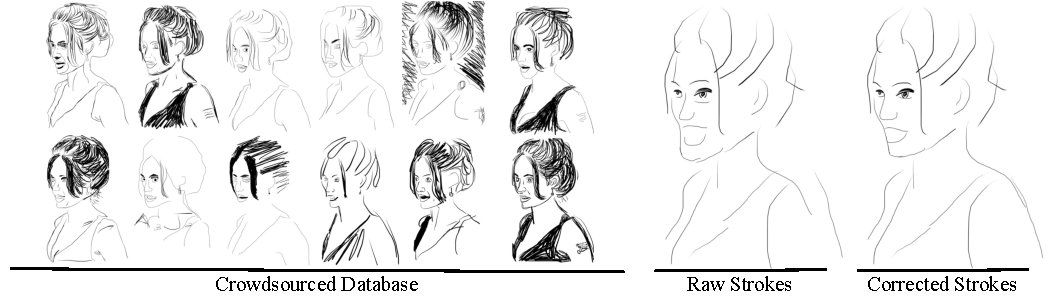
\includegraphics[width=7in]{figures/AngelinaHeader.pdf}
 \caption{ Left: twelve examples of drawings of Angelina Jolie, created by DrawAFriend players.  Right: our algorithm automatically corrects new drawings in real-time based on a consensus of the drawings by previous players.}
 \label{fig:teaser}
}

\maketitle


\begin{abstract}
% The big data revolution is profoundly transforming computer science
% and society. Problems which frustrated generations of researchers,
% such as machine translation and object recognition, suddenly became
% ``solved'' when run on large datasets. However, the scarcity of data
% in many domains threatens the continued success of the big data
% approach. We now see a schism between domains for which large
% datasets are available (such as translation corpuses) and those for
% which it is not, with much more rapid progress in the former. We
% propose a method of collecting new datasets through crowd sourcing
% and social game mechanics. First, we assemble a corpus of aligned
% drawings via a new iPhone game, {\em DrawAFriend} developed
% specifically for the purpose of collecting drawing data. Second, by
% analyzing the database of drawings, we build a spatially varying
% model of artistic consensus at the stroke level. Using this model,
% we introduce a surprisingly simple method to improve strokes in
% real-time. Importantly, our auto-corrections appear nearly invisible
% to the user, while seamlessly preserving artistic intent. Lastly, we
% use the game itself to evaluate the effectiveness of our stroke
% correction algorithm. We do this by randomly turning on stroke
% correction for half our player base, and AB testing how
% auto-correction effects their drawings.

We propose a method for the large-scale collection and analysis of
drawing through crowdsourcing. {\em
DrawAFriend} is a new iPhone game developed specifically for the
purpose of collecting drawing data. Analyzing the database of
drawings, we build a spatially varying model of artistic consensus
at the stroke level. We leverage this model to present a
surprisingly simple stroke-correction method to improve strokes in
real-time. Importantly, our auto-corrections run interactively and
appear nearly invisible to the user, while seamlessly preserving
artistic intent. We use the game itself to evaluate the
effectiveness of our stroke correction algorithm.

\end{abstract}

\newcommand{\theKeywords}{Interactive Drawings, Crowdsourcing,}

\keywords{\theKeywords}\keywordlist % <<>>  Also add to hypersetup ?

%% These CR lists are pointless and just waste space.
%\begin{CRcatlist}
%  \CRcat{I.3.7}{Computer Graphics}{Three-Dimensional Graphics}{Animation};
%  \CRcat{I.6.8}{Simulation and Modeling}{Types of Simulation}{Animation}.
%\end{CRcatlist}

% \TOGlinkslist  %<<>> Add this later

%\abovecopyrightspacetext{Contact email: Anonymous review.} %<<>>
\copyrightspace

% put useful definitions here that we can include throughout the paper

\newcommand{\etal}[1][\ ]{{et~al\@.}#1}

% macro for writing DrawAFriend
\newcommand{\daf}[0]{\emph{DrawAFriend}~}
\newcommand{\imgtbl}[1]{\includegraphics[width=0.5in]{figures/imagetable/#1.png}}
\newcommand{\imgtblpdf}[1]{\includegraphics[width=0.5in]{figures/imagetable/#1.pdf}}

\newcommand{\adrien}[1]{\textcolor{NavyBlue}{AT:#1}}
\newcommand{\alex}[1]{\textcolor{ForestGreen}{AL:#1}}
\newcommand{\michael}[1]{\textcolor{OrangeRed}{MC:#1}}
\newcommand{\nico}[1]{\textcolor{LimeGreen}{NF:#1}}
\section{Introduction}

Drawing as a means of communication dates well before other forms of
recorded history. Today, drawing remains a vital form of artistic
expression and an important window into human perception. However,
the central challenge to further scientific analysis of drawing is
data scarcity. Although search engines index a huge collection of
line drawings, these images are stored in raster format with little
or no useful metadata. Ideally, a drawing corpus would contain
precise stroke-level data for each image, including timing
information. We would also like semantic metadata identifying
artists and subjects. Even more ambitiously, we would like to glean
\emph{perceptual} information, such as which strokes most
contributed to image recognition. Finally, for statistical purposes,
we would like a \emph{large} dataset, with many drawings by the same
artist and many drawings of the same subject by different artists.

To address this challenge, we developed \emph{DrawAFriend}, an
iPhone game specifically designed to collect drawing data, including
all of the information described above. We currently focus on face
portraits. Such drawings are exceedingly difficult to draw by hand,
and even more so using a touch interface on a small mobile device.
To aid users and to collect multiple drawings of the same subject,
we allow players to trace over existing photographs. In its first
week of release \daf generated over 1,500 images per day.

As a first application, we demonstrate how the \daf corpus can be
mined to provide a self-correcting touch-based drawing interface on
mobile devices. We observe that drawing with a touch device often
suffers from the ``fat finger'' problem. We conceptually factor this
issue into two elements: (1) the ``intent'' of the artist in drawing
a stroke, and (2) an additional random noise component caused by
inaccuracy in the touch interface. We therefore hypothesize that if
we can determine a consensus of strokes (in an appropriate sense)
over a sufficiently large database of drawings, then we can cancel
out the noise and recover the artist's original intent. This allows
us to develop a real-time {\em self-correcting} touch interface: in
essence, we clean up the artists drawing as they draw by using data
from hundreds of previous drawings of the same subject. We analyze
these images to compute a \emph{correction vector field} that for
any location, points towards a nearby consensus of strokes. We
further introduce a surprisingly simple method to correct strokes
based on this consensus while maintaining the {\em stylistic}
choices of the artist. The interface requires no new user
interaction paradigms, in other words, it appears ``invisible'' to
the user. The resulting strokes feel more like the intent of the
user than the raw original strokes.

To validate the the effectiveness of our auto-correction algorithm,
we ran a large-scale user study within the game. Each time a
user draws a celebrity, we randomly turn the auto stroke correction
on or off. Our results validate the effectiveness of our stroke
correction algorithm: with autocorrect on, artists do not need to
draw as accurately, and they undo their strokes less. The ability of
\daf to serve equally simultaneously as a large-scale visual data
collection platform, and as a statistically relevant user study
underscores the generality of our crowdsourcing approach.

%\adrien{We need a few sentences or a paragraph hear explaining how
%we have only begun to explore the trove of information contained in
%this corpus, indicating that we conclude by sketching some further
%applications of this data. Much of this can come from the rebuttal,
%I think.}  -- this is in the rebuttal do we want it in the end

%We do actually have this at the very end is that enough? It makes sense to close off the paper like that...

% hrough the use of crowd sourcing, we develop a novel
% way of understanding how people draw. First we construct a game,
% {\em DrawAFriend}, that encourages people to draw. Second, we use
% the corpus of drawings from previous players to aid new drawers to
% overcome the fat finger problem by auto-correcting strokes by
% attracting them towards the consensus of strokes in previous
% drawings while leaving their individual styles intact. This
% application represents only a first use of a new dataset of hand
% drawings collected by the game. Lastly we use the {\em DrawAFriend}
% game itself to evaluate the effectiveness of our stroke correction
% algorithm by dividing users into two groups, with and without
% auto-correction on.
% 




% The big data revolution is profoundly transforming computer science
% and society. Problems which frustrated generations of researchers,
% such as machine translation and object recognition, suddenly are on
% the brink of becoming ``solved'' when run on large datasets. We now
% see a schism between domains for which large datasets are available
% such as translation corpuses and those for which it is not,
% with much more rapid progress in the former.
%
% One domain suffering from such data scarcity is hand-drawn images.








%Our use of a game to generate data brings the added challenge that
%the game must be rewarding and encourage repeated play. We address
%this challenge by allowing players to draw mutual friends on the
%as well as celebrities. We phrase the challenge as a
%guessing game, with the important corollary that we can learn
%\emph{when} a particular face was recognized, i.e. which strokes
%were necessary for recognition.




%%%%%%%%%%%%%%%%%%%%%%%%%%%%%%
% Adrien's Old Section Below %
%%%%%%%%%%%%%%%%%%%%%%%%%%%%%%

% The big data revolution is profoundly transforming computer science
% and society. Problems which frustrated generations of researchers,
% such as machine translation and object recognition, suddenly became
% ``solved'' when run on large datasets. However, the scarcity of data
% in many domains threatens the continued success of the big data
% approach. We now see a schism between domains for which large
% datasets are available – such as translation corpuses – and
% those for which it is not, with much more rapid progress in the
% former.
%
% One domain suffering from such data scarcity is hand-drawn images.
% Visual expression is a fundamental human trait with deep connections
% to perception and creativity, yet most of our understanding of the
% drawing process is purely qualitative.  Given this
% state of affairs, a great many fascinating questions about human
% drawing cannot be answered quantitatively. An ideal drawing corpus
% would be annotated by artist and subject allowing us to measure
% variation in ``drawing style'' across a single subject, while
% illumination how one artist's style varies across subjects. Another
% goal would be to have precise stroke-level data, including timing
% and order. Such stroke information could allow us to rigorously
% answer questions about the order in which artists draw lines, and
% how quickly. We might even glean semantic knowledge about the
% subject by understanding the temporal relationships among strokes.
% Going further, drawings are meant to be recognized and understood by
% others. Ideally, a drawing corpus could shed light on these issues,
% for example: which strokes were most salient in conveying the
% subject? Finally, for statistical purposes, we would like a
% \emph{large} dataset, with many drawing by the same artist and many
% drawings of the same subject.
%
% To address these issues, we have developed an iPhone game called
% \emph{DrawAFriend}, which is intended to generate millions of
% hand-drawn images containing all of the information described above.
% In comparison with previous work which studied simple line drawings
% \adrien{[cite Hayes and Shadowdraw]}, we focus on face portraits.
% Such drawings are exceedingly difficult to draw by hand, and even
% more so using a touch interface. Therefore, we decided to allow
% players to trace over existing photographs. Even within this
% restricted setting, we observe startling variation in drawing style
% \adrien{maybe this should be the teaser image?}. Moreover, when
% multiple artists trace the same face, we get the added benefit that
% all drawings are in geometric correspondence, which can lead to much
% simplified analysis. In contrast to previous work which generated
% drawings through Amazon Mechanical Turk, our use of a game to
% generate data brings the added challenge that the game must be
% rewarding and encourage repeated play. We address this challenge by
% allowing player to draw mutual friends on the social network as well
% as celebrities. We phrase the challenge as a guessing game, with the
% important corollary that we can learn \emph{when} a particular face
% was recognized, i.e. which strokes were necessary for recognition.
% The success our game design is born out in the numbers: within
% DrawAFriend's first \textbf{X} days on the market, we generated
% \textbf{Y} images, all with stroke-level information.
%
% We believe that the completely new, data-rich corpus generated by
% this game will allow us to solve numerous fascinating questions,
% including those delineated above. In this paper, we focus on
% studying how such a large database can help us create
% self-correcting touch-based interactions on mobile devices. We
% observe that drawing with a touch device often suffers from the
% ``fat finger'' problem. We factor this issue into two elements: (1)
% the ``intent'' of the artist in drawing a stroke, and (2) an
% additional random noise component caused by inaccuracy in the touch
% interface. We therefore hypothesize that if strokes are ``average''
% (in an appropriate sense) over a sufficiently large database of
% drawings, then we can cancel out the noise and recover the original
% intent. Furthermore, this data can allow us to develop a
% ``self-correcting'' touch interface: in essence, we can clean up the
% artists drawing in real time by using data from hundreds of previous
% drawings of the same subject. To solve this problem, we present a
% new metric for ``local stroke coherence,'' that is, regions of the
% images where many artists agree. We further present a surprisingly
% simple method to correct strokes based on this metric making it
% significantly easier to draw faces.
%
% More generally, we consider the DrawAFriend corpus to be a
% significant contribution which will benefit research by the graphics
% community, and we hope that our game design insights might guide
% other researchers seeking to collect large datasets in domains
% suffering from data scarcity.


% - fat finger problem	
% 	- althogh we believe
% 	- with applications from automated graphic training to
% 	
%
% 	- problem with drawing using touch interfaces
% 	- naively we can use zooming but this isn't fun
% 	- how can we leverage many drawings
% 	- our insight: average strokes are good
%
% 	- this simple method can clean up many strokes,
% 	- more generally
% 		- valuable corpus which we will make available to the community
% 		- and will also yield design patterns
% 		which we can reuse to incentivize large groups to generate further
% 		datasets,
%
% To solve this problem, my research uses social networking mechanism
% to elicit large datasets that have never been assembled before. As a
% model problem, I am working on human drawing.  Nonetheless, recent work by my colleagues and I
% shed light on the power of computation to illuminate fundamental
% aspects of this process. At Princeton, I worked on a highly cited
% SIGGRAPH paper which computationally analyized line drawings. To
% achieve this result however, we painstakingly set up workshops where
% artists would draw pre-selected objects. The dataset itself only
% included 208 line drawings from 29 artists. This work inspired my
% collaborators to develop ShadowDraw, which demonstrated that large
% image datasets can be leveraged a real-time free-hand drawing
% guidance software which leverages a large database of images from
% the internet. Unsupervised learning on thousands or millions of
% drawings would be groundbreaking. The creation of this dataset was
% not possible until Facebook integration and my project, DrawAFriend.

% \adrien{Note we got over 5,000 images in the first three days of the game.} 
\section{Related Work}

The graphics community is witnessing a recent spike of interest in
``big data'' approaches to understanding drawing, with the
prototypical examples being \emph{ShadowDraw} \cite{Lee:2011} which
help guide freeform sketching and \emph{WhatsMySketch}
\cite{Eitz:2012:HSO} which identifies iPhone sketches as one of 250
possible object classes. A important distinction between these
efforts and our work is the data-collection approach. Lee \etal used
30,000 sketches downloaded from existing web databases in raster
format which Eitz \etal collected 20,000 sketches on Amazon
Mechanical Turk (https://www.mturk.com). By contrast created a
publicly available iPhone game \emph{DrawAFriend} which uses
mechanics similar to \emph{DrawSomething}
(http://omgpop.com/drawsomething) to intrinsically motivate players
to contribute drawings. Therefore, rather than sequestering data
collection into an initial phase of our research, we collect data
continuously with zero marginal cost per user, and can re-instrument
the game to change data collection on the fly. Our game approach
also gives us more information per user, including knowledge of
their social graph, but requires us to design a compelling game to
collect data. In this sense, \daf is closer to the games of von Ahn
and colleagues \shortcite{vonAhn:2004:LIC,vonAhn:2006:PGL} which
uses games to label objects in images. By contract, we ask players
to complete the much more complex (and creative) task of actually
drawing new images. Another important distinction is that \emph{ShadowDraw} and
\emph{WhatsMySketch} study freeform sketching, while our celebrity
database consists of many registered drawings of the same image.

There has also been considerable work in the Human Computer
Interaction community on solving the problem of inaccurate touch
interactions, often called the \emph{fat finger problem}. Wigdor
\etal \shortcite{Wigdor:2009:RUP} taxonomized touch-based
interaction errors, and presented novel visual cues to help the user
understand their intent. Other work has addressed the fat finger
problem by designing new interaction patterns
\cite{Albinsson:2003:HPT,Benko:2006:PST,Forlines06hybridpointing,Vogel07shift:a},
or adding additional interaction hardware
\cite{Scott:2010:RTE,Wigdor:2006:UTI,Wigdor:2007:LTS}. The book by
Benko and Wigdor \shortcite{Benko:Fatfinger} presents a good
overview of work in the field.

By contrast, we add no additional hardware, visual cues or
interaction paradigms. Instead we use data from lots of previous
drawings of the same image to seamlessly correct user strokes as
they draw. Our stroke correction approach draws inspiration from the
work of Cole \etal \shortcite{Cole:2008:WDP}, which studied
collected statistics on a small number of hand-collected, registered
sketches of the same object. Our stroke correction method was
inspired by the finding of Cole \etal (confirmed by our data) that
artists frequently draw similar lines. We further develop this this
idea with our hypothesis that the average of these strokes
represents the fundamental user ``intent'' towards which we snap
strokes. Our approach minimizes an energy function on the stroke
similar to the intelligent scissors method
\cite{Mortensen:1995:ISF}. However, rather than snap to image
contours \adrien{Note: it would be interesting to have this as a
comparison.}, our energy function is based on average strokes from
many registered sketches. We further preserve stroke geometry using
a Laplacian method which is often used in geometry processing
\cite{Sorkine:2004:LSE}. Another system called \emph{iCanDraw}
\cite{Dixon:2010:IUS} helps users draw faces, although using a
tutorial approach rather than looking at automatic correction based
on a large dataset.

% 
% [ ] Intelligent Scissors :: 
% 	[ ] Intelligent Scissors (a.k.a. Live Wire or Magnetic Lasso)
% 	[Mortensen and Barrett 1995] allows a user to choose a “minimum
% 	cost contour” by roughly tracing the object’s boundary with the
% 	mouse. A
% [ ] Laplacian Mesh Editting ~
% 

\section{DrawAFriend: The Game}

\begin{figure}
  \centering%
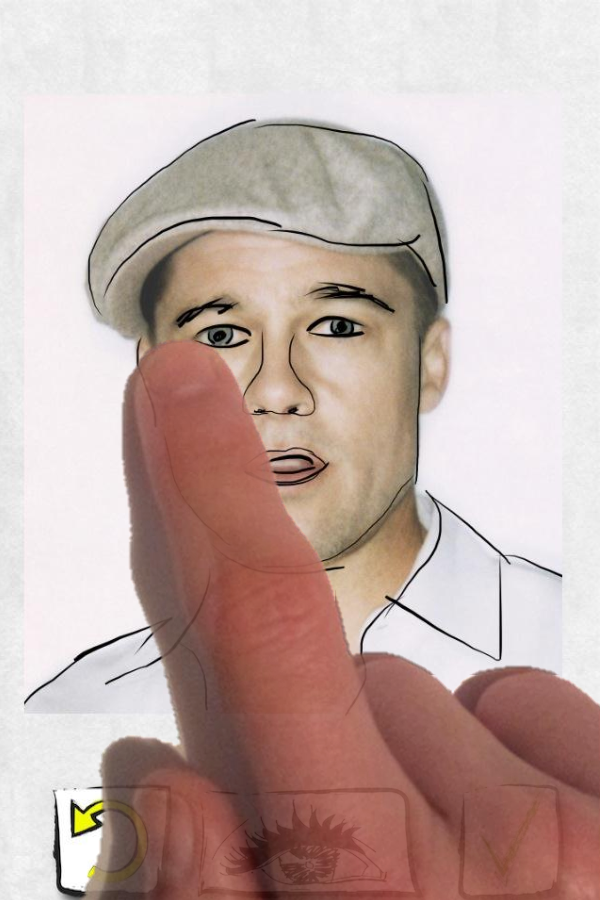
\includegraphics[width=1.5in]{DaF/PicHand2.pdf}
\hspace{0.1in}
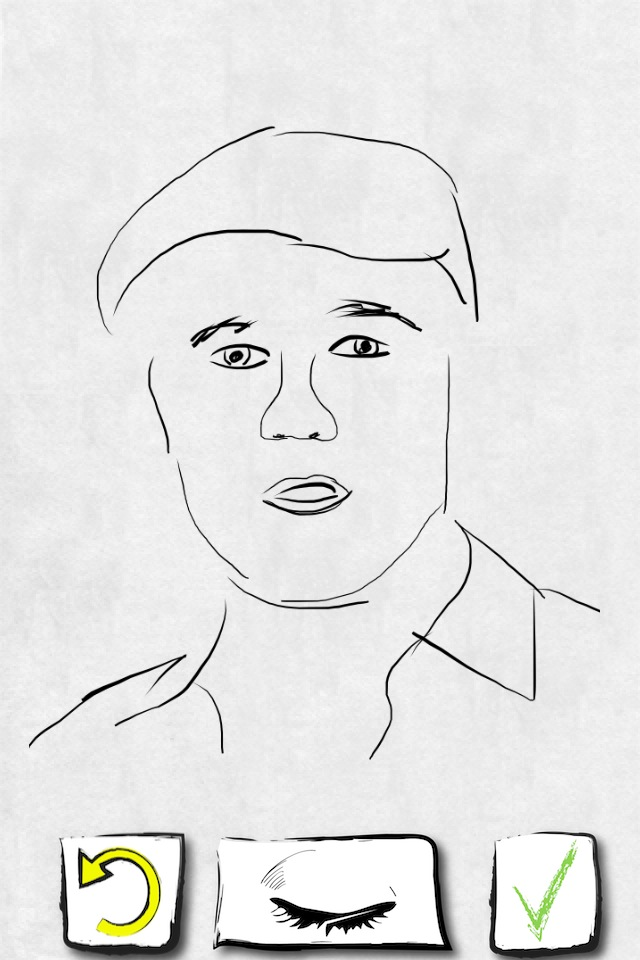
\includegraphics[width=1.5in]{DaF/IMG_3044.jpg}
  \caption{DrawAFriend: tracing a photo (left), the drawing alone (right).}
  \label{fig:DaF}
\end{figure}

\begin{figure}
  \centering%
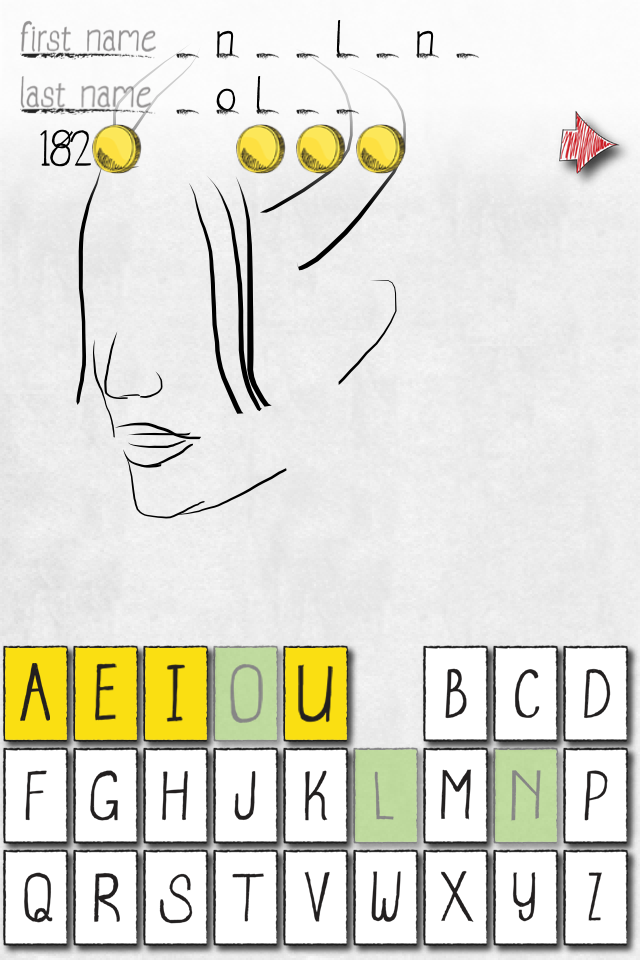
\includegraphics[width=1.5in]{DaF/angelina_guess1.png}
\hspace{0.1in}
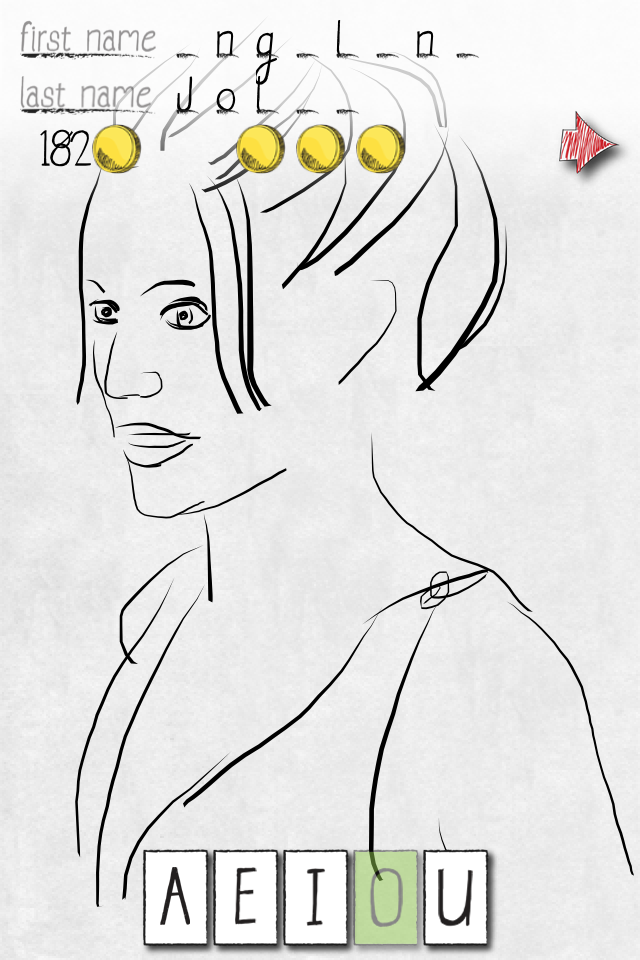
\includegraphics[width=1.5in]{DaF/angelina_guess2.png}
  \caption{DrawAFriend: guessing identity (left). Once a player guesses all consonants in a name, the consonant keys animate away and vowels no longer cost coins. (right).}
  \label{fig:DaF2}
\end{figure}

We have developed DrawAFriend, a Facebook-integrated turn-based drawing and guessing game for mobile devices.  It works as follows. Players have an option to start a game with either a Facebook friend or a random other player.  The player is then given four pictures which he can draw. These will either be mutual Facebook friends' profile pictures or  celebrity photos. In the case of a random player, only celebrity photos are offered to draw.

After choosing a photo to draw, the player is brought to the drawing screen. There she can trace the image (see Figure~\ref{fig:DaF} left). At any point, the user can press the {\em eye} button to hide the photo and see their drawing on its own (Figure~\ref{fig:DaF} right). To overcome the limitations of the phone's size, and touch screen inaccuracies, players can pan and zoom using the pinch zoom, and two fingered pan gestures.

Once finished, the player sends her drawing to the friend or random player with whom she is playing. The friend receives a notification that they have a drawing to guess. Once the drawing is complete, the user is prompted to guess the identity of the other player's drawing (Figure~\ref{fig:DaF2} left). The user sees a replay of the drawing being made, and similar to {\em Hangman}, the player can guess which letters are in the mutual friend or celebrity's name. Vowels originally cost coins, however once all the consonants are guessed the final vowels are offered for free to complete the guess (Figure~\ref{fig:DaF2} right).

This tracing paradigm results in a set of pre-aligned drawings. Whereas other papers begin with rasterized versions of drawings, we collect individual strokes represented as polylines along with timing information.  Furthermore, by observing the guesses we can indirectly evaluate the quality of the drawings. We hypothesize that a good drawing is much more likely to be guessed correctly than a bad drawing. DrawAFriend thus leverages a dataset of quality photos (Faceboook profile pictures and celebrity images) and via the efforts of players, results in a large dataset of user created drawings. This dataset includes drawings from artists around the world with different artistic and cultural backgrounds.

For the purposes of tackling the fat finger problem, we focus for the remainder of the paper on the corpus of celebrity drawings. These represent sets of drawings of the same photographs by many different artists. That said, not all drawings are created equal. While we did not want to pass judgment on different styles, certain drawings appear to be random scribbles by people simply trying out the game. We manually removed these from our database, and selected an average of 100 drawings per celebrity. 

\section{Data Driven Drawing}

Our goal is to provide a drawing interface on mobile devices that provides the feeling that the user is in full control, while simultaneously providing assistance, in particular, to overcome the inherent fat finger problem. As described earlier, the problem is more constrained than a general drawing system through the use of a tracing paradigm. The simplest idea would be to attract drawn strokes to edges found in the image being traced. Unfortunately, this idea fails in two respects. First edge detectors such as Canny methods (see Figure~\ref{fig:edges}, left) have no notion of semantics and thus appear noisy and inconsistent. Second, unlike automated edge detectors, humans tend to select only the most meaningful edges to draw.

\begin{figure}
  \centering%
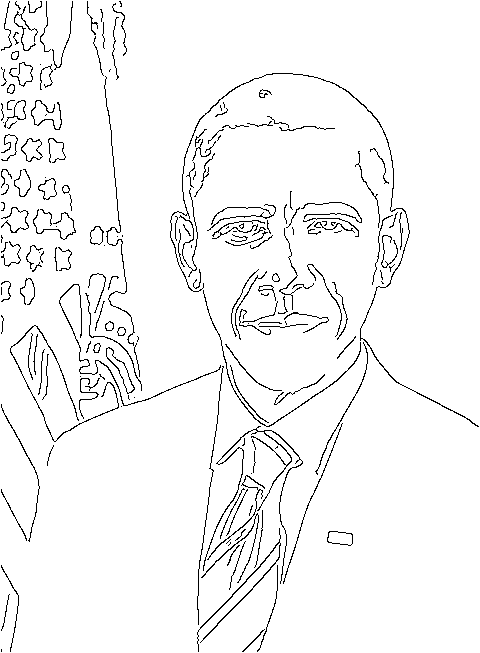
\includegraphics[height=2in]{figures/imagetable/edges_bo.png}
\hspace{0.1in}
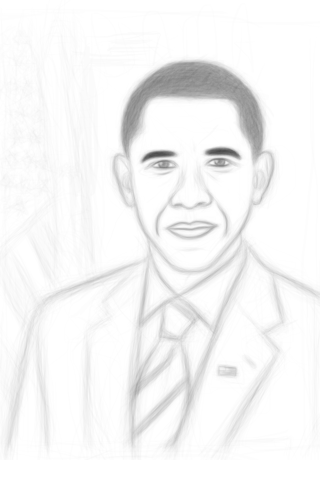
\includegraphics[height=2in]{figures/imagetable/avg_bo.png}
  \caption{Left: Canny edges, Right: average of the rasterized drawings. Neither of these serves as a simple means to correct strokes due to noisy edges (Canny), and fuzzy and inconsistent edges (average).}
  \label{fig:edges}
\end{figure}

To provide assistance, we take advantage of previous drawings of the same face and then pull the users strokes towards a {\em consensus} of strokes from previous drawings. The simplest idea for forming a consensus would be to use an {\em average} drawing (see Figure~\ref{fig:edges}, right). This idea is also very problematic as the averages tend to create very fat lines of varying darkness, as well as broad regions such as in the hair. Although some kind of {\em skeletonization} may aid the first problem, it would fail on the second.

Instead, we develop a stroke correction strategy with two phases.

\textbf{(i) Consensus Finding:} Using the training drawings available for an image, we create a correction vector field, which indicates for each pixel on the image, the delta toward the nearest {\em consensus stroke}.  This phase is run off-line.

\textbf{(ii) Interactive Correction:} The correction vector field is transmitted to the mobile device along with the image to be traced.  When a user draws a stroke, the field is sampled, and the stroke is moved in real-time in a way that maintains the original style.

\subsection{The Correction Vector Field}

%\begin{figure}
%  \centering%
%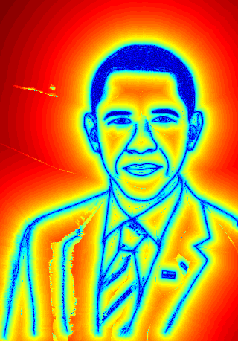
\includegraphics[height=2in]{figures/imagetable/mag_bo.png}
%\hspace{0.1in}
%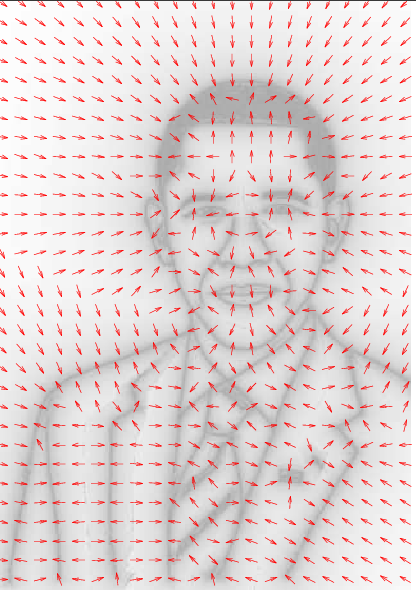
\includegraphics[height=2in]{figures/imagetable/dir_bo.png}
%  \caption{Left: vector magnitude, Right: sampled vector field orientations}
%  \label{fig:vectorfield}
%\end{figure}

A correction vector field, $V(p)$, (see Figure~\ref{fig:image-table}(c)and (d)) is constructed to point, for each location $p$ in the image, towards the nearest {\em consensus}. Intuitively , the consensus represents a location where many almost parallel strokes pass nearby in the training drawings. Interestingly, we do not need to construct an explicit model of consensus strokes. Instead, we can directly compute $V$ using a modified version of the {\em mean shift} algorithm~\cite{10.1109/ICCV.1999.790416}.


\begin{figure}
  \centering%
  \includegraphics[width=3.2in]{ellipse.png}
  \caption{A didactic blow-up of the graphs in Figure 6. The point at the origin represents a point, $p$ on a stroke being drawn. The red points are the set of nearest stroke neighbors from each database drawing. Note that the orientation of the strokes are always orthogonal to a vector from the origin. We determine a correction vector based on a learned anisotropic Gaussian with mean $\mu$ and sigmas $\sigma_1$ and $\sigma_2$ surrounding a mode of nearby points from strokes in the database drawings.}
  \label{fig:ellipse}
\end{figure}

\begin{figure}
  \centering%
  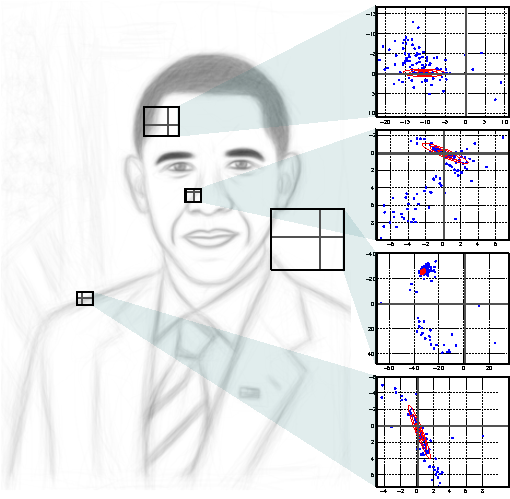
\includegraphics[width=3.2in]{figures/nearest-neighbor-plots.pdf}
  \caption{Nearest neighbors and learned Gaussians for four points in the Obama dataset.  The Gaussian distribution is shown with ellipses at the first, second, and third standard deviations.}
  \label{fig:neighbors}
\end{figure}


Given a point $p$ on a stroke in the image being drawn, we first find the nearest stroke point, $v_i$ in each drawing, $D_i$, in our training set. We place the nearest points, $v$, in a coordinate system using $p$ as the origin (see the red points in Figure~\ref{fig:ellipse} and the points in Figure~\ref{fig:neighbors}). One key observation is that the position of the point $v_i$ also implicitly encodes the orientation of the nearest stroke in $D_i$. In particular, the stroke orientation will be orthogonal to the vector $v_i$ (unless the nearest point is a stroke endpoint). Otherwise there would be some closer point along the stroke. Thus, if the nearest strokes from different users are closely aligned in position and orientation, they will produce a set of the nearest points, $v$, that lie approximately along a line. Furthermore, this line will intersect the origin (i.e., the point $p$). We use this observation to build the consensus of nearby strokes.

Our goal is find a consensus of nearby strokes that avoids undue influence from outliers. For the points, $v$, we seek a {\em mode} in which the points lie in close proximity to each other and lie roughly along a line pointing back towards the origin. We employ an iterative mean shift style algorithm for the mode finding.

Our algorithm works by iteratively updating a vector of weights, {\bf w}, which represent the belief that a particular nearest point, $v_i$, is a member of the consensus stroke. The final correction vector, $V(p)$, is determined by the weighted mean of the points, $v$. We initialize all weights using a symmetric Gaussian centered at the origin, with $\sigma$ equal to the mean distance to all nearest points, $v$.

The iterations proceed by determining an anisotropic Gaussian with weighted mean, ${\bf \mu} = \left(\sum_j w_j {\bf v}_j\right) / \sum_j w_j$, with
$\sigma_1$ in the direction back toward the origin (equation~\ref{sig1}), and ($\sigma_2$) in the orthogonal direction (equation~\ref{sig2}). 
%The mean is given by:
%\begin{equation}
%{\bf \mu} = \left(\sum_j w_j {\bf v}_j\right) / \sum_j w_j  \label{mean}
%\end{equation}
%and 
We define the normalized mean vector as, ${\bf \nu} = \mu/||\mu|| $,
and finally determine the anisotropic standard deviations of the projected distances to the mean, given by
\begin{eqnarray}
\sigma_1 =  \sqrt{\left(\sum_j w_j (({\bf v}_j-\mu)^{\bf T}\nu)^2\right) / \sum_j w_j} \label{sig1}\\
\sigma_2 =  \sqrt{\left(\sum_j w_j ({\bf v}_j^{\bf T}\nu_\perp)^2\right) / \sum_j w_j} \label{sig2}
\end{eqnarray}
We add a simple regularization $w_i \leftarrow w_i/ (w_i+0.05)$ to the weights.  The regularization serves to reinforce points near the mean, and further discount points away from the mean. The term 0.05, which intuitively says that any points more than two standard deviations away from the mean are mostly noise, was chosen experimentally. We then reweight all points according to the new Gaussian distribution, and iterate until the mean stops moving.

The system typically converges quickly (all of our experiments use a hard-coded 10 iterations), and $V(p)$ is set to $\mu$.  Examples of nearest neighbor sets and their resulting consensus strokes are shown in Figure \ref{fig:neighbors}.

\subsection{Real-time Stroke Correction}


The vector field, $V$, defined above indicates a best guess of how any individual vertex, $p$, on a stroke polyline should move to match the consensus of all drawings.

The naive approach is to take the points $(p_1, \ldots, p_k)$ comprising a stroke, along with their correction field samples $(V(p_1), \ldots, V(p_k))$, and directly move each point to arrive at $(p_1 + V(p_1), \ldots, p_k + V(p_k))$.  Unfortunately, noise and discontinuities in the vector field cause undesirable end results. More importantly, any {\em stylistic} choices such as intentional wiggles inherent in the original stroke would also be lost.  We hypothesize that the fat finger problem is likely to cause the input stroke to be off by a roughly constant displacement, while the original stroke shape is likely to represent the user's {\em intent}.

Our goal is thus to use the guidance of the vector field on where to move, but still maintain most of the shape of the original stroke.  We therefore create and solve an over-constrained linear system that represents both of those objectives.

With $p_i$ representing input stroke sample locations for $i=1\ldots k$, $V_i$ a shorthand for $V(p_i)$ representing the correction vector field at $p_i$, and $p_i'$ representing the corrected samples, we construct a quadratic error function as:

\begin{equation}
E =  \sum_{i=1}^k (p_i' - (p_i + V_i))^2 +  \alpha \sum_{i=2}^k ((p_i' - p_{i-1}') - (p_i - p_{i-1}))^2
\end{equation}

The first term represents the faithfulness to the correction vector field. The second term tries to maintain the shape of the stroke by enforcing that neighboring points move in sync. The $\alpha$ term weights the relative importance of the two terms. The error is minimized with respect to p' using a standard least squares solver.


\subsubsection{Setting $\alpha$ - Closely Spaced Consensus Strokes}

A higher $\alpha$ value results in {\em stiffer} strokes in the sense that they maintain their shape instead of following variations in the vector field precisely. Aside from maintaining the {\em style} of the strokes, a high stiffness also helps avoid having part of a stroke pulled in one direction and another part pulled in another. This can happen especially when there are two closely spaced parallel lines in the consensus, such as the two sides of the nose, or the bottom and top of the lips. Unfortunately, such a very high $\alpha$ does not allow the strokes to adapt at all to the subtleties of the consensus drawing represented in the vector field.

To achieve the dual goals of avoiding the two nearby stroke problem while balancing stiffness and style, we use a {\em continuation method}, performing three iterations of the solver described above. We begin with $\alpha=10$. This high stiffness value leads to an almost rigid transformation of the stroke to the most dominant consensus region. We then lower $\alpha$ to 7, and feed the previous result, $\hat{p}$ into the first error term, $(p_i' - (\hat{p}_i + V_i))$, while keeping the original terms for the latter half of the error measure, and solve the new system. We repeat this one final time with $\alpha=4$ to get our final result. The $\alpha$ values (10, 7, and 4) were chosen experimentally.

\subsubsection{Purely Stylistic Strokes}

We also found that some strokes are purely stylistic in nature. For example, someone writes ``Obama'' above the president's head. We do not want such strokes to have parts pulled towards the consensus. We make a binary decision about whether the stroke is purely stylistic, in which case, we leave it alone. A stroke is defined to be purely stylistic if either of two conditions is met. Either the maximum vector length, $\max_i||V_i)||$, is greater than $5mm$ (approximately $1/10^{th}$ the screen width), or a stroke's direction is mostly orthogonal to the vector field. The latter term is measured with the average of absolute cosines $\frac{1}{N}\sum_i||N(p_i - p_{i-1}) \cdot N(V(p_i))||\textrm{,}$ where $N(\cdot)$ normalizes vectors. If the average falls below 0.5, the stroke is considered purely stylistic.






\section{Results}
\begin{figure}
  \centering%
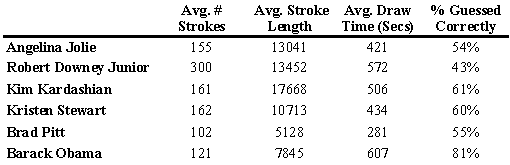
\includegraphics[height=1.1in]{./figures/daf-stats-cropped.pdf}
  \caption{Celebrity drawing statistics for 611 hand-picked drawings from the first four days after launch.}
  \label{fig:daf-stats}
\end{figure}


\begin{figure}[!t]
  \centering%
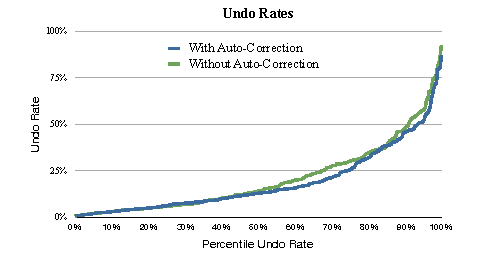
\includegraphics[width=3.5in]{./figures/userstudy/undoRates_chart_cropped.pdf}
  \caption{This chart plots the undo rates (percentage of all strokes that are undone, i.e., undoes / undoes + not-undoes) for
each drawing sorted by undo rates. The X axis indicates the percentile undo rate, for example at the 50\% mark half of the
drawings had less undoes and half more. As can be seen the two sets behave similarly for the first half in which the undo
rate is below about 15\%. However for higher percentiles the two sets diverge, with the auto-corrected drawings generally
showing lower undo rates.}
  \label{fig:daf-undos}
\end{figure}



After smaller-scale trials, \emph{DrawAFriend} was released publicly on January 8th, 2013. In 88 days there were 14,270 drawings. After the launch of \emph{DrawAFriend}, our project proceeded in three phases. First we collected drawings for six celebrities to prime our initial correction vector field. Second we use the correction field to add an automatic stroke correction helper into the game. Lastly we crowd sourced the evaluation of our stroke corrector, by AB testing it within the game.

\subsection{\daf Correction Vector Field}
In order to integrate the correction vector field into the game, we needed to prime it with initial drawings. In four days players had downloaded the game over 2000 times and created 6373 drawings. In that time, players had already spent approximately 10 full 24 hour days drawing. We used these drawings to create the correction vector field.


Players were given the option of drawing Facebook friends or one of an initial set of six celebrities: Robert Downey Jr.\footnote{Meritano, E. ``Robert Downey Jr.'' Photo. wikimedia.org. Apr 2008.}, Angelina Jolie\footnote{Natt, C. ``Angelina Jolie.'' Photo. wikimedia.org. Jun 2007.}, Kim Kardashian\footnote{Shankbone, D. ``Kim Kardashian.'' Photo. wikimedia.org. May 2005.}, Barack Obama\footnote{Souza, P. ``Barack Obama.'' Photo. wikimedia.org. Jan 2009.}, Brad Pitt\footnote{Boyd, B. ``Brad Pitt.'' Photo. wikimedia.org. Mar 2008.}, or Kristen Stewart\footnote{Dispara, A. ``Kristen Stewart.'' Photo. wikimedia.org. Oct 2008.}. From the drawings generated in the first four days, we manually chose 611 celebrity drawings. We filtered by picking drawings in which players had made an attempt to accurately draw the eyes (the most intricate feature to draw). These 611 drawings were slightly less than 10\% of the dataset. The rest of the dataset mostly consisted of drawings that players had drawn quickly, resembling a person like scribble. While this portion of the dataset could be used for analysis, we did not train our correction vector field on it.  Figure \ref{fig:daf-stats} references statistics for these 611 drawings.

\begin{figure}[!t]
  \centering%
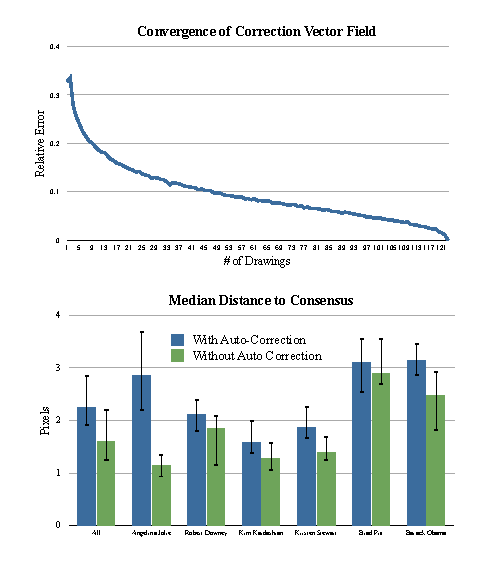
\includegraphics[width=3.5in]{./figures/userstudy/twoGraph.pdf}

  \caption{Top: Convergence of the correction vector field as more
images are added. Relative error is measured between the correction
vector field built using X drawings and the correction vector field
using all 124 drawings. (The final dip is an artifact caused by
measuring convergence to a specific vector field computed with 124 drawings rather than to the ``true'' limit correction field. This is also why the error drops down to zero exactly.) Bottom: The median
across drawings of the mean distance of stroke points to the
consensus for each celebrity with and without auto- correction.
Distance is measured by the value of the correction vector field
under the strokes. The error bars mark the 60th and 40th percentile
for each celebrity. Auto-correction universally leads to a greater
distance, implying that users can be sloppier when auto-correction
is activated.}

  \label{fig:daf-two}
\end{figure}

\begin{figure*}[!t]
  \centering%
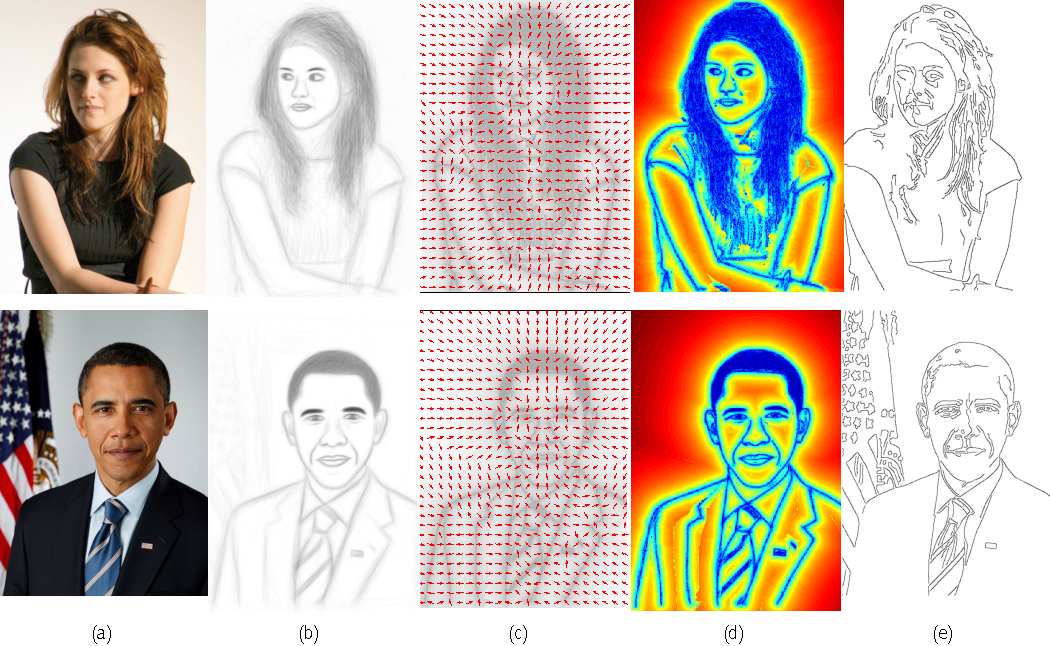
\includegraphics[width=7in]{./imagetable/kristenAndObama.pdf}

%\vspace{-0.35in}
  \caption{DrawAFriend users draw one of six celebrities (a). We use our database of hundreds of drawings per subject -- shown averaged in (b) -- to precompute a \emph{correction vector field} (c) enabling real-time drawing assistance on the iPhone. The magnitude of our vector field (d) reveals a consensus of artistic renderings strikingly different than what we could compute with automated methods, such as a canny edge detector (e).}
 % \vspace{-0.25in}
  \label{fig:image-table}
\end{figure*}

\vspace{+0.25in}
We ran our modified mean shift algorithm on this initial dataset to create the correction vector fields shown in Figure \ref{fig:image-table}. Our MATLAB implementation took under 5 minutes for each celebrity.  The great majority of the time was spent in un-optimized nearest neighbor search. The dimensions of the correction vector field are 460x320. In Figure \ref{fig:daf-two} (top) we plot how our correction vector field converges for Brad Pitt. We do this by calculating the relative error between the vector field for a subset of the drawings and the vector field for all 124 drawings. There appears to be an inflection point around 25 drawings, where the correction vector field would probably work well. However every additional drawing still improves the correction field, implying that after 124 drawings it has not completely converged. We can also use the correction vector field to filter our drawings. Drawings whose points were on average 10 pixels away from the consensus were never actually portraits (most often they were the celebrity's name spelt out). We use this filtering method to exclude non-portraits in the user study described below.

\subsection {Drawing Enhancements}



We apply the correction vector field to interactively modify strokes during the drawing process. For every new stroke point added, a background thread is spun off to correct the new stroke. Once the thread completes if newer points have accumulated another thread is immediately spun off. Without adding user interface elements to the existing \daf UI, we seamlessly integrate stroke auto-correction. As the user draws, strokes are subtly corrected at interactive rates on an iPhone 4. In general, the fact that corrections are being applied is almost invisible to the user. Instead, strokes appear where the user {\em intended} to draw.

%????Please see the \alex{Not sure how to reference the teaser on top} and the video for interactive examples.

We also applied the correction vector field retrospectively to improve the existing database of user drawings. The drawings are already quite good, making the vector field corrections all the more impressive.  While the algorithm improves the images, it does so without sacrificing style. For comparisons of the raw drawings and the corrected images please see Figure~\ref{fig:results}, our video, and the supplementary files.

\subsection {Crowdsourced User Study}

One key advantage of developing \daf as an online game is the ability to quickly deploy a study of users at scale. To test the effectiveness of the stroke auto-correction, we instrumented the game to enable a simple AB study. Every time a user started a drawing they were unknowingly placed in one of two groups. One group drew the celebrities as before. The other group (unbeknownst to them) drew with the stroke auto-correction on. By comparing these two groups, we can assess the effectiveness of the stroke auto-correction helper. Users drew one of the six celebrities. We use the consensus vector field to filter out drawings that could not be portraits. We record the geometry and timing of each stroke, all {\em undo}s, and the recognition rates of the players receiving the drawings.

% By adding only a couple of lines of code, we transformed a data collection crowd sourcing system into a large-scale user study.


\subsubsection {User Study Results}

After approximately one week, 500 players had ``contributed'' over 1,300 drawings to the user study. Using this data we assess recognition rates (measuring how good the drawings are from the perspective of others). We also analyze undo rates (providing an insight into how artists like their own drawings). Finally we measure average ``distance'' from the artistic consensus (measuring how carefully artists are drawing).

%Our results show that autocorrect reduced undo rates (the ratio of undos to all other strokes). This effect is magnified for careful drawers (who undid 30\% or more strokes). Their undo rates decreased by a significant 5\% (Wilcoxian p-value = .045).  Before we analyzed the undo rates we removed all drawings that had 0 undos (assuming most of these players did not know undo existed) and all drawings with less than 10 strokes (assuming these drawings were not actual attempts to draw the celebrity).  Figure \ref{fig:daf-three} middle shows the effect that auto correction has on decorating undo rates, particularly for more careful drawers. We view the drop in undo rates as an improvement in how players view their own drawings.

%[Someone Please Review this Paragraph]

First we investigate {\em undoes} as an indication of how artists like their own drawing. Since players used a different number
of strokes, we focus on undo rates, which is the number of strokes undone over the total number of strokes. For example if
a user drew 100 strokes and pressed undo for 40 of them, this would have an undo rate of 40\%. For our analysis we removed
all drawings that had 0 undoes (assuming that this implied players did not know undo existed). This left 327 drawings auto-corrected
 and 295 that were not. We sorted each set of drawings by the undo rates from lowest to highest, and in Figure
\ref{fig:daf-undos}, plotted the undo rate for each percentile of sorted drawings (this normalizes for the different
number of drawings in each set). The distribution of undo rates for drawings with fewer undoes track together for both
sets with and without autocorrection. However the undo rates diverge further along the sorted lists. This seems to imply
that our auto-corrector lowers the undo rate for more careful drawers (players that undo a larger percent of their
strokes).

 
With auto-correct on,  we observe a significant increase in the average distance between the actual uncorrected strokes
and the consensus drawings (as measured by the \emph{correction vector field}). We perform a two-sample Wilcoxon test of
whether or not there is a difference in the mean of the correction vector field under the stroke points with auto correct
on versus off. This shows a significant difference in the means, with a p-value of $1.653 \times 10^{-6}$.  This suggests that
artists do not need to draw as precisely. Figure \ref{fig:daf-two} (bottom) shows the median distance to the consensus for
each celebrity with a sample size of 570 auto-corrected and 533 not auto-corrected.
 

Interestingly, statistical analysis reveals that the auto-corrector does not significantly alter recognizability.
Corrected drawings had a recognition rate of $37.5\% \pm 2.02\%$ while uncorrected drawings had an average recognition
rate of $38.6\% \pm 2.11\%$ (again 570 and 533 drawings respectively). Running a permutation we get a p-value = .87, which implies that the two populations are uncharacteristically similar. We believe that our auto-corrector does not change
players final drawing quality. Rather it makes reaching this level of quality easier by requiring less undoes and less
accuracy.

\begin{figure*}[!t]
  \centering%
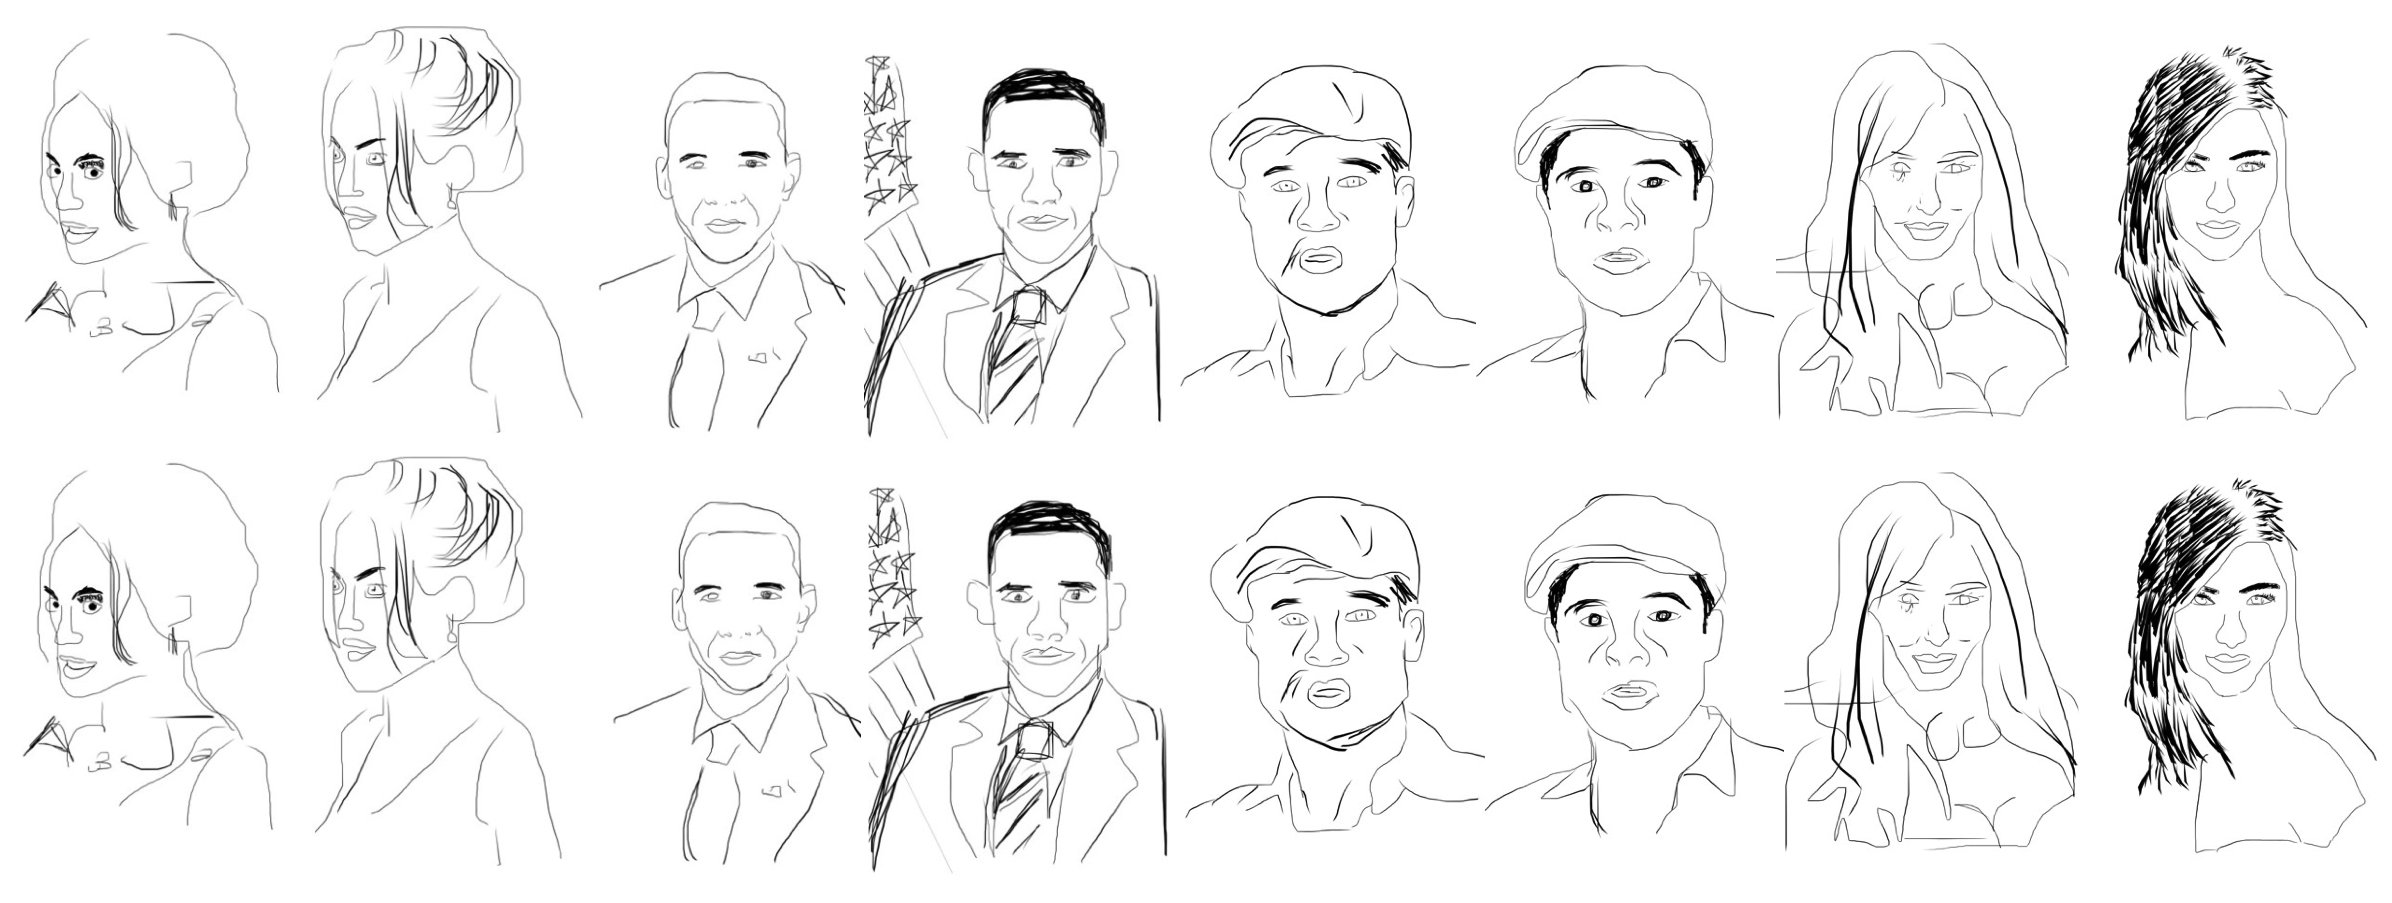
\includegraphics[width=7in]{./figures/ResultsAll_16.pdf}
\vspace{-0.35in}
  \caption{Celebrity drawings: original strokes (bottom rows) and after automatic adjustment to consensus (top rows). (Please see the supplementary files for more examples and also for an interface so you can flip between them.)}
\vspace{-0.25in}
  \label{fig:results}
\end{figure*}

\section{Conclusion}

This paper presented a unique crowdsourcing approach to address the
``fat finger'' problem in touch-based drawing. We developed an
iPhone game, \emph{DrawAFriend}, specifically for the purpose of
collecting drawing data. We then introduced a method to extract
stroke-level artistic consensus from a large drawing corpus. The
resulting \emph{correction vector field} improves strokes in
real-time without new interactions interfaces, while preserving artistic
intent (see video). We presented stroke correction on over 80 images (supplemental
materials) which illustrate our method's ability to improve both
aesthetics and recognizability. 

In the future, we are excited to
quantify these improvements by releasing stroke correction to the
public and measuring drawing speed and recognizability. In general,
we believe that DrawAFriend presents an unprecedented platform to
perform quantitative drawing analysis at the Internet scale.

Our stroke correction method has several drawbacks. Even with stroke
correction, many drawings are still not beautiful. We would like to
study automatic aesthetic enhancement of strokes, including weight
and texture. We also see several avenues to improve and generalize
our correction vector field model. For example, the field depends on
2D position only. An anisotropic field, however, could correct strokes
differently based on their orientation. We plan to {\em lift} the correction field to
3D (position plus orientation). This could be especially
beneficial at stroke intersections which we do not explicitly model
at present. Nevertheless, we have found that our simple isotropic
field corrects strokes well in practice, especially
around dominant lines for which there is great artistic consensus.
Moving beyond the single consensus model, we envision automatically
identifying and clustering by artistic ``style''. This would allow new drawings to
be enhanced based on which style they most closely mimic to provide more
nuanced stroke correction.

Stroke correction represents just the tip of the iceberg for 
applications of the large (and
growing) DrawAFriend image corpus. Thus far, we have explored only a
small portion of the trove of data we are collecting. For example,
measuring how quickly drawings are identified could shed light on
which strokes are most salient for recognition. Studying when the
user undoes strokes could provide clues as as to which strokes are
good or bad. Analyzing stroke order could enable us to predict what
the artist will draw next, potentially enabling completely new
drawing interactions. Making this data available to the community,
we hope to explore both these exciting ideas, and discover as-yet
unknown applications of this rich dataset.

%  expect to find yet
% more exciting applications for this new drawing corpus.

%
%
% when images are guessed correctly
%
% - whether they guessed quickly and how long
% 	- use this as weights for the consensus.
% 	- which were most
%
% For example, we could study
%
% are using only a
% small portion of the data
%
%  Rigorous analysis of the data
% could provide insight into how people draw specific facial features,
% in what order do artists draw strokes, and which strokes
%
% First, we assemble a corpus of aligned drawings via a new iPhone
% game we developed specifically for the purpose of collecting drawing
% data.
%
% Such stroke
% information could allow us to rigorously answer questions about the
% order in which artists draw lines, and how quickly.
% 	
% - we want to learn a lot more from these drawings
% 	- how to people draw eyes
% 	- what order do they draw strokes
% 	- what will they draw next?
%
%
% - things that the game tells that we're not yet exploiting
% 	- how
% 	- where they zoom
%
%
% - future work
%
% 	- 

%\section*{Acknowledgments}
%
%Removed for anonymous review.

%----------------------------------------------------------------------------
% Acknowledgements
%----------------------------------------------------------------------------
\renewcommand{\abstractname}{Acknowledgements}
\begin{abstract}
 This work was supported by an NSF Graduate Research Fellowship, an NSF Career Award (IIS0953985), and by generous gifts from Google, Qualcomm, Adobe, Intel, and the Okawa Foundation. Thank you to Larry Zitnick. Also special thanks to Erdmuthe Limpaecher, Katherine Miller, Jackie Bello, Paul Kompfner, and Sam Grossberg for playtesting.
\end{abstract}


%----------------------------------------------------------------------------
% Bibliography
%----------------------------------------------------------------------------

\bibliographystyle{TexInputs/acmsiggraph}
\bibliography{drawafriend}

%----------------------------------------------------------------------------


\end{document}
% \end{input}
